\chapter{Fase sperimentale}
\fancyhead[RO, LE]{\bfseries Fase sperimentale}
Dopo aver introdotto le nozioni teoriche necessarie, possiamo finalmente passare alla parte sperimentale di questa tesi. Verrà descritto l'ambiente di sviluppo fino ad arrivare all'analisi dei risultati ottenuti, con i relativi grafici.

\section{Qiskit e la IBM Quantum Experience}
La piattaforma che ho utilizzato durante i vari esperimenti prende il nome di Qiskit (Quantum Information Science Kit): un framework open-source per la computazione quantistica fondato da IBM Research.

Ciò che ha spinto l'azienda a sviluppare uno strumento di questo tipo, insieme ed altre istituzioni accademiche, riguarda l'accesso al loro servizio di Cloud Quantum Computing denominato IBM Q Experience.
L'obbiettivo è quello di mettere a disposizione macchine quantistiche a favore di tutta la comunità scientifica, toccando con particolare interesse alcuni settori di ricerca; queste macchine possono essere liberamente utilizzate sia per scopi di ricerca che a puro scopo didattico.

La versione principale e più utilizzata di Qiskit è basata sul linguaggio Python, attraverso il quale si possono creare programmi basati sulla rappresentazione Open-QASM \cite{larose2019articolo, assembly2017articolo} dei circuiti quantistici.

Richiamando all'occorrenza delle apposite API \cite{qiskit2018articolo} è possibile comunicare con i dispositivi IBM, così da far eseguire porzioni di codice a macchine reali o simulatori, i quali permettono di ottenere i risultati ideali.
Il servizio IBM Q Experience può essere utilizzato all'interno del sito, senza bisogno di installare nessun pacchetto.
Quest'ultimo mette a disposizione diversi esempi per avvicinarsi a questi temi, che variano dal più semplice al più complesso; è inoltre presente una piattaforma grafica chiamata Circuit Composer in cui è possibile realizzare circuiti trascinando elementi.

Nella Tabella \ref{table:dispositivi_quantistici} è possibile vedere alcuni dei backend disponibili gratuitamente, con relativo numero di qubit.
\begin{table}[h]
\centering
\begin{tabular}{l|c|c}
    \hline\hline
    \textbf{Nome macchina} &  \textbf{Num.qubits} & \textbf{Simulatore}\\
    \hline
    \textit{ibmq\_santiago} & 5 &  \\
    \textit{ibmq\_athens} & 5 &  \\
    \textit{ibmq\_vigo} & 5 &  \\
    \textit{ibmq\_valencia} & 5 &  \\
    \textit{ibmq\_16\_melbourne} & 15 &  \\
    \textit{ibmq\_ourense} & 5 &  \\
    \textit{ibmq\_qasm\_simulator} & {Up to 32} & $\times$\\
    \hline\hline
\end{tabular}
\caption{Alcuni dei dispositivi IBM disponibili.}
\label{table:dispositivi_quantistici}
\end{table}
\newline\newline

Una volta creati e lanciati gli esperimenti, l'utente dovrà attendere un lasso di tempo che potrà essere influenzato o meno dalla coda presente nel dispositivo.
La complessità dell'esperimento avviato richiederà a sua volta una mole di tempo variabile per essere portato a termine.

\subsection{Elementi di Qiskit}
Qiskit\footnote{Qiskit: An Open-source Framework for Quantum Computing, 2019, \url{https://doi.org/10.5281/zenodo.2562111}}  è una libreria di Python dedicata al calcolo quantistico, suddivisa in quattro grandi sotto-librerie, ognuna con un ambito ben preciso e specifico, come si può evincere dalla Figura \ref{fig:elementi_qiskit}.
\begin{itemize}
    \renewcommand\labelitemi{--}
    \item \textbf{\textit{Terra}}, fornisce una base per la creazione di programmi quantistici a livello di circuiti ed impulsi, definendo inoltre le interfacce utilizzabili dall'utente finale il quale potrà comunicare con i dispositivi remoti;
    \item \textbf{\textit{Aer}}, ci aiuta a comprendere i limiti dei processori classici dimostrando fino a che punto possono imitare il calcolo quantistico, include al suo interno vari simulatori scritti in C++ ottimizzati per l'esecuzione di circuiti compilati in Terra, consentendo inoltre di verificare se i computer attuali e futuri funzionino correttamente;
    \item \textbf{\textit{Ignis}}, è pensato per coloro che vogliono progettare codici di correzione degli errori quantistici, permettendo una migliore caratterizzazione degli stessi ed un perfezionamento delle porte durante l'elaborazione in presenza di rumore;
    \item \textbf{\textit{Aqua}}, racchiude al suo interno una serie di algoritmi quantistici che trovano applicazioni nel mondo reale, in particolare i domini d'interesse risultano essere la chimica, l'ottimizzazione, la finanza e l'intelligenza artificiale.
\end{itemize}
\begin{figure}[htp]
    \centering
    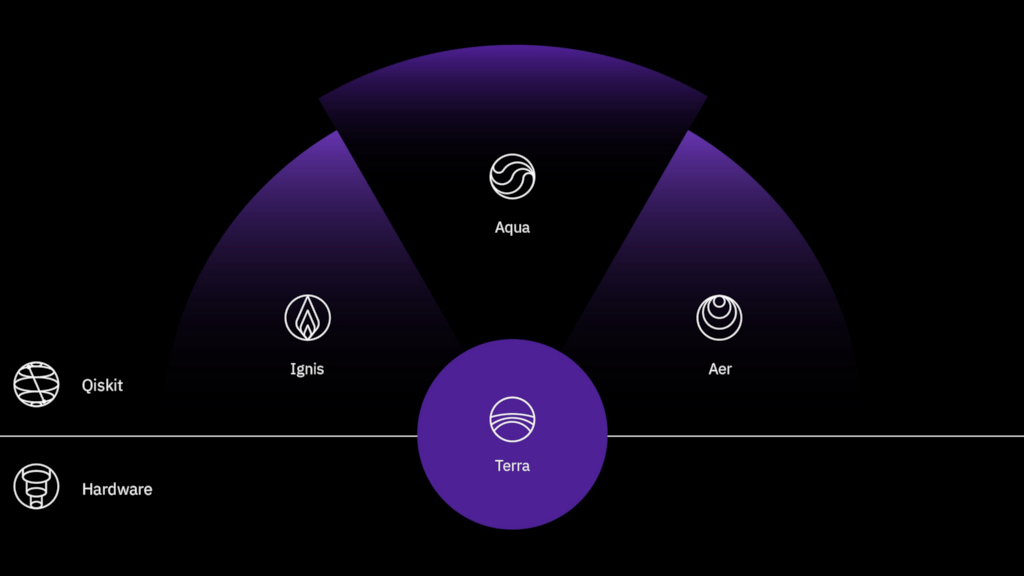
\includegraphics[width=13cm]{Images/Capitolo3/elementi_qiskit.png}
    \caption{Schema elementi di Qiskit.}
    \label{fig:elementi_qiskit}
\end{figure}

\section{Descrizione del sistema}
Come abbiamo visto nel Paragrafo \ref{subsec:vqe}, per implementare l'algoritmo VQE è necessario definire un circuito parametrico quantistico.
Quest'ultimo ci permette di effettuare la stima energetica della molecola presa in esame attraverso il susseguirsi di operazioni, specificate da porte logiche quantistiche.

Ora andremo ad analizzare in dettaglio i due circuiti utilizzati, sia dal punto di vista grafico che strutturale.
\subsection{TwoLocal}
Il circuito TwoLocal è parametrizzato in quanto costituito da strati di rotazione alternati e strati di entanglement.
Le rotazioni vengono specificate attraverso porte a qubit singolo ed applicate su tutti i qubit, lo strato di entanglement invece, utilizza porte a due qubit per intrecciare quest'ultimi secondo una delle seguenti strategie: \textit{full}, \textit{linear}, \textit{circular} e \textit{sca}.

Si può vedere una sua rappresentazione con full entanglement in Figura \ref{fig:circuito_twolocal}.
\begin{figure}[htp]
    \centering
    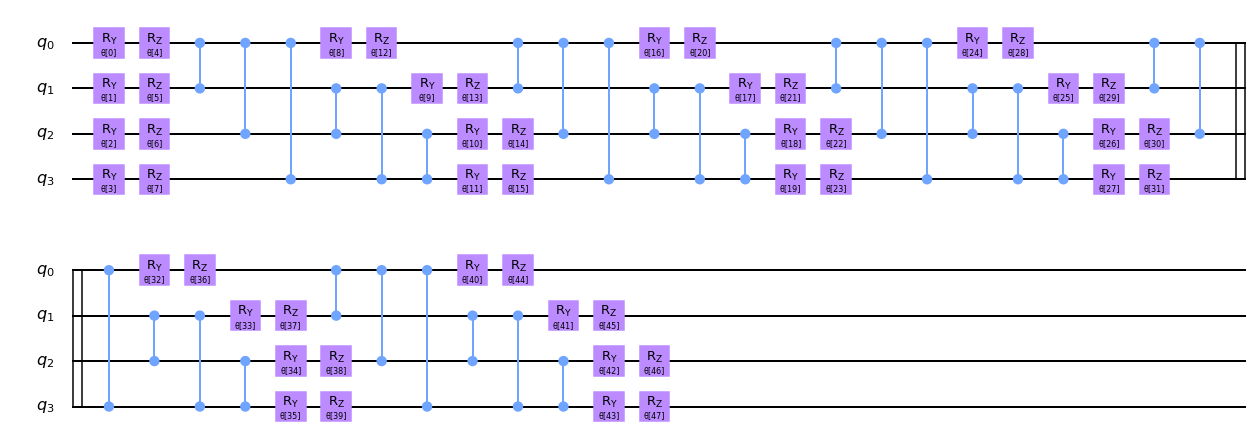
\includegraphics[width=13cm]{Images/Capitolo3/circuito_twolocal.png}
    \caption[Schema circuito TwoLocal.]{Schema circuito TwoLocal con full entanglement e porte logiche RY, RZ e CZ.}
    \label{fig:circuito_twolocal}
\end{figure}

\subsection{EfficientSU2}
Il circuito EfficientSU2 è costituito da strati di operazioni a qubit singolo, attraversato da intrecci SU(2) e $CX$ entanglement.
Questo è un modello euristico che può essere utilizzato per preparare funzioni d'onda di prova per algoritmi quantistici variazionali o circuiti di classificazione per l'apprendimento automatico.

SU(2) sta per gruppo unitario speciale di grado 2, i suoi elementi sono matrici unitarie $2\times2$ con determinante uguale a 1, come le porte di rotazione di Pauli.

Si può vedere una sua doppia rappresentazione, la prima in Figura \ref{fig:circuito_efficientsu2_linear} con linear entanglement mentre la seconda in Figura \ref{fig:circuito_efficientsu2_full} con full entanglement.
\begin{figure}[htp]
    \centering
    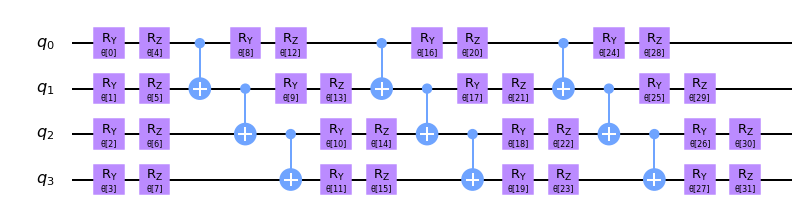
\includegraphics[width=12cm]{Images/Capitolo3/circuito_efficientsu2_linear.png}
    \caption{Schema circuito EfficientSU2 con linear entanglement.}
    \label{fig:circuito_efficientsu2_linear}
\end{figure}
\begin{figure}[htp]
    \centering
    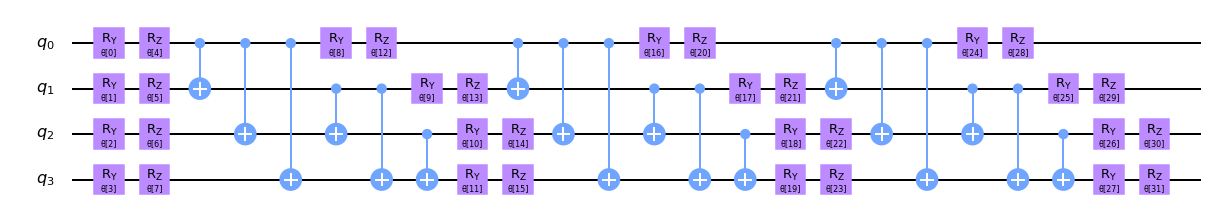
\includegraphics[width=13cm]{Images/Capitolo3/circuito_efficientsu2_full.png}
    \caption{Schema circuito EfficientSU2 con full entanglement.}
    \label{fig:circuito_efficientsu2_full}
\end{figure}
\newline

\section{Passaggi preliminari}
\subsection{Preparazione dell'ambiente di sviluppo}
Per utilizzare Qiskit è necessario avere installato nel proprio terminale il linguaggio di programmazione Python, versione 3.5 o successive; si ha inoltre piena compatibilità con i più diffusi sistemi operativi (Windows, macOS e Linux).
Il modo migliore per utilizzare questo framework è quello di installare un ambiente virtuale all'interno della propria macchina locale o su cloud, così da separare Qiskit dalle altre applicazione ed avere un'esperienza d'uso migliore.

I passi da me svolti per preparare l'ambiente di sviluppo nel sistema operativo Ubuntu sono stati quindi i seguenti:
\begin{enumerate}
    \item installare Anaconda e creare un ambiente minimale con solo Python al suo interno;
    \begin{itemize}
        \item[$\$$] \mintinline{bash}{conda create -n name_of_my_env python=3}
    \end{itemize}
    \item attivare l'ambiente appena creato;
    \begin{itemize}
        \item[$\$$] \mintinline{bash}{conda activate name_of_my_env}
    \end{itemize}
    \item installare Qiskit tramite il gestore dei pacchetti di Python (pip);
    \begin{itemize}
        \item[$\$$] \mintinline{bash}{pip install qiskit}
    \end{itemize}
    \item utilizzare Jupyter Notebook per interagire con Qiskit ed iniziare a svolgere i primi esperimenti.
\end{enumerate}

\subsection{Autenticazione all'IBM Quantum Systems}
Abbiamo visto come IBM metta a disposizione il suo servizio di Cloud Quantum Computing denominato IBM Q Experience, per utilizzarlo e configurarlo correttamente con Qiskit ho dovuto seguire i passi qui in elenco:
\begin{enumerate}
    \item creare gratuitamente un account IBM Q Experience;
    \item navigare nella sezione \say{My Account} e copiare il token disponibile nella casella di testo, così da poter accedere all'API;
    \item eseguire questi comandi in Jupyter per archiviare localmente il token API, sostituendo MY\_API\_TOKEN con il valore copiato;
    \begin{itemize}
        \item[] \mintinline{python}{from qiskit import IBMQ} \\
                \mintinline{python}{IBMQ.save_account('MY_API_TOKEN')}
    \end{itemize}
\end{enumerate}

\section{Analisi del problema}
Come già accennato in precedenza, si cercherà di utilizzare l'algoritmo ibrido VQE, all'interno un sistema quantistico simulato ideale, denominato da Qiskit \textit{statevector}.

Al fine di poter confrontare i dati ed i grafici ottenuti da queste simulazioni si è deciso di applicare allo stesso problema un algoritmo classico, chiamato NumpyMinumEigenSolver, il quale utilizza a sua volta l'operatore Hamiltoniano per ricavare i valori dell'energia di legame.

Il problema, analizzato principalmente a livello teorico da chi studia chimica computazionale, ci ha permesso di misurare l'energia propagata da una molecola in funzione dell'interdistanza atomica tra gli atomi costituenti.

La molecola sulla quale sono stati fatti il maggior numero di esperimenti è l'Idrogeno ($H_2$) essendo la più semplice a livello di struttura, mentre un numero inferiore di esperimenti è stato fatto anche per l'Idruro di Litio ($LiH$), il quale ha richiesto tempi di esecuzione molto più lunghi.

Le prime simulazioni sono state fatte utilizzando il backend denominato BasicAer, scritto in Python ed attualmente definito obsoleto, per questo motivo si è poi passati all'utilizzo del backend Aer, scritto in C++ e perciò più prestante.
Il metodo di simulazione specificato per entrambi i backend è stato \textit{statevector\_simulator}; a seconda della configurazione scelta ho potuto aggiungere l'opzione \textit{statevector\_gpu} al fine di utilizzare la potenza di calcolo della scheda video.

Una volta decisi questi parametri è stato necessario scegliere un ottimizzatore locale, ossia una funzione che tenta di trovare un valore ottimale all'interno di un range; quello su cui è stato fatto il maggior numero di prove è L\_BFGS\_B ma ne sono stati testati anche altri.

\subsection{Risultati ottenuti}
Le macchine che sono state utilizzate per effettuare i test sono 3; ne verranno elencate di seguito le caratteristiche sia hardware che software e ad ogni configurazione verrà associato un nome identificativo.
\small
\begin{itemize}
    \item \textbf{Notebook\_CPU} - Ubuntu 19.10 - i7-8750H - 16GB
    \item \textbf{Notebook\_GPU} - Ubuntu 19.10 - i7-8750H - GTX 1050 Ti - 16GB
    \item \textbf{Colab\_CPU} - Linux - Backend Google Compute Engine - 12.72GB
    \item \textbf{Colab\_GPU} - Linux - Backend (GPU) Google Compute Engine - 12.72GB
    \item \textbf{Tower\_GPU} - Windows 10 v2004 build 20236.1005 - Ubuntu 20.04 on WSL2 - i5-6600K - GTX 1070 - 16GB
\end{itemize}
\normalsize

Ogni tabella nella prima riga evidenzia il nome identificativo del dispositivo ed il backend utilizzato; se il dispositivo avrà come sigla finale \say{CPU} l'opzione specificata sarà \textit{statevector}, altrimenti nel caso di \say{GPU}, verrà utilizzata l'accelerazione hardware attraverso la direttiva \textit{statevector\_gpu}.

Se non diversamente specificato si farà riferimento a test svolti sulla molecola d'Idrogeno $H_2$ ed i tempi di esecuzione verranno indicati secondo lo standard ISO 8601 (hh:mm:ss,ms).

Ogni grafico sarà formato da due curve che rappresentano rispettivamente i differenti metodi utilizzati per calcolare l'energia di legame.
In azzurro si ha la curva definita attraverso il metodo d'approssimazione d'onda di Hartree-Fock, il quale minimizza l'energia totale presente all'interno della molecola; in arancione si può vedere invece la curva generata da uno dei due algoritmi da noi utilizzati: NumPyMinimumEigensolver o VQE.
Nei punti in cui il valore dell'ordinata raggiunge il suo estremo inferiore ci troveremo nello stato fondamentale della molecola, ovvero il punto in cui l'energia contenuta in essa è minima, da qui in poi le due curve risulteranno simili con variazioni assunte nelle coordinate $y$.

\subsubsection{L\_BFGS\_B}
L'obiettivo di Broyden-Fletcher-Goldfarb-Shanno Bound a memoria limitata è di minimizzare il valore differenziabile di una funzione scalare $f$.

Questo ottimizzatore non richiede l'hessiana di $f$ (la matrice delle derivate seconde di $f$) quando si tenta di calcolare il valore minimo della funzione, bensì effettua una stima iniziale del valore ottimale e procede iterativamente per perfezionare tale stima con una sequenza di stime migliori, risolvendo così problemi di ottimizzazione non vincolata e non lineare.

Nel nostro caso andremo ad eseguire un massimo di 2500 valutazioni di funzioni.

%-------------------------------------------------------------------------------------------------------
% NumPyMinimumEigensolver
\begin{figure}[htp]
    \centering
    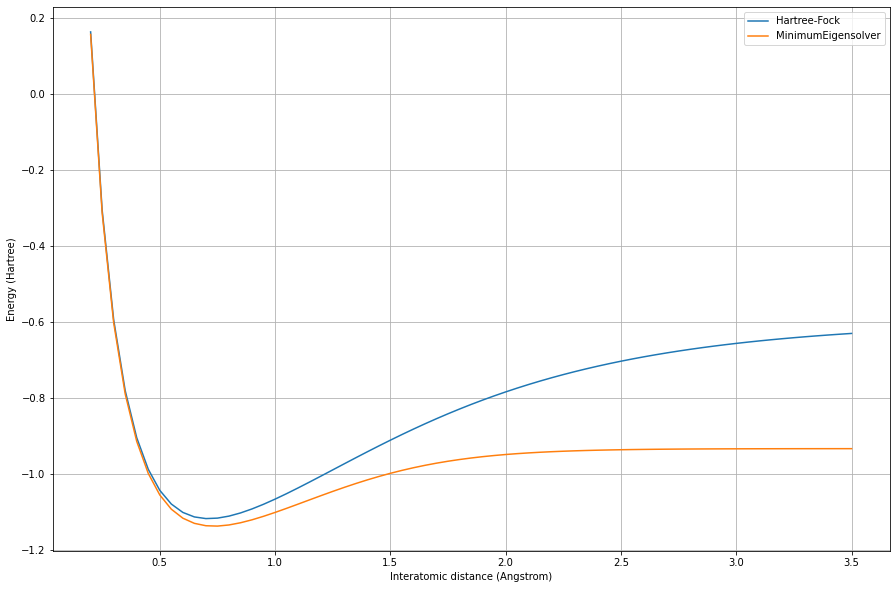
\includegraphics[width=8cm]{Images/Capitolo3/Plots/H2_numpy_minimum_eigensolver_plot.png}
    \caption[Grafico atteso \newline H2 NumPyMinimumEigensolver.]{}
    \label{fig:numpy_minimum_eigensolver}
\end{figure}
\noindent
\newline
Il grafico mostrato in Figura \ref{fig:numpy_minimum_eigensolver} rappresenta il risultato atteso, ottenuto attraverso il metodo del calcolo degli autovalori dell'Hamiltoniano utilizzando l'algoritmo classico NumPyMinimumEigensolver.
\newline
%-------------------------------------------------------------------------------------------------------
% PRIMO TEST - Notebook_CPU - BasicAer
\begin{minipage}[b]{0.39\textwidth}
    \scalebox{0.8}{%
    \begin{tabular}[b]{l|c}
        \hline\hline
        \multicolumn{2}{c}{\textbf{\textit{Notebook\_CPU - BasicAer}}}\\
        \hline
        \multirow{3}{*}{\textit{TwoLocal}} & 33:49,7277235984804\\
        \cline{2-2} & 32:36,4913177490235\\
        \cline{2-2} & 33:08,7257981300354\\
        \hline\hline
    \end{tabular}}
    \captionsetup{type=table}
    \caption[Risultati prima simulazione.]{Nella colonna di destra sono riportati i tempi di esecuzione.}
    \label{table:notebookcpu_basicaer}
\end{minipage}
\hfill
\begin{minipage}[b]{0.59\textwidth}
    \centering
    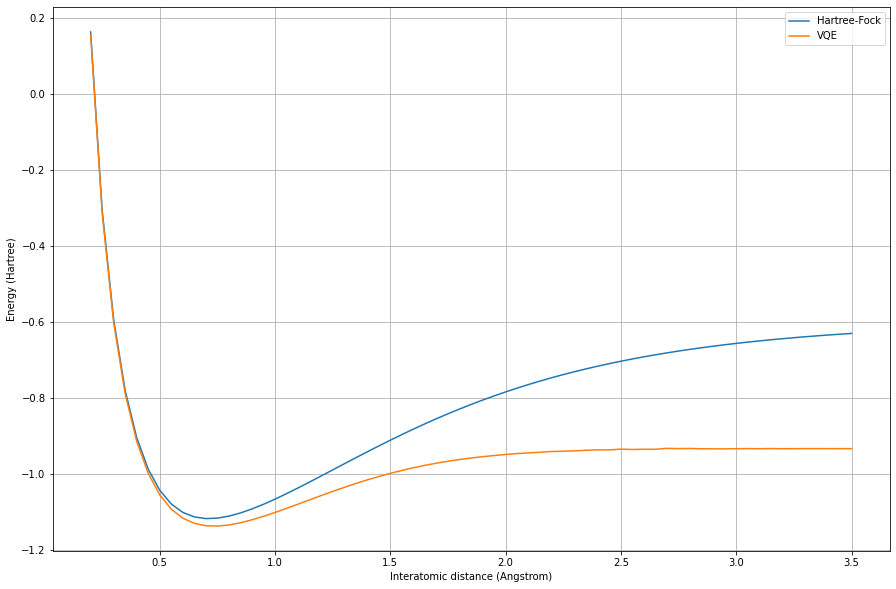
\includegraphics[width=1.0\textwidth]{Images/Capitolo3/Plots/H2_twolocal_ry_rz_cz_basic_cpu_plot.png}
    \captionof{figure}[Grafico 1 \newline TwoLocal - L\_BFGS\_B - Notebook\_CPU - BasicAer.]{}
    \label{fig:notebookcpu_basicaer}
\end{minipage}
\noindent
La prima simulazione è stata eseguita su Notebook\_CPU, con circuito TwoLocal e backend BasicAer.
Nella Tabella \ref{table:notebookcpu_basicaer} possiamo notare come i tempi di esecuzione hanno superato di poco la mezz'ora ed il grafico risultante, mostrato in Figura \ref{fig:notebookcpu_basicaer}, è praticamente identico a quello desiderato.
%-------------------------------------------------------------------------------------------------------
% SECONDO TEST - Notebook_CPU - Aer
\begin{minipage}[b]{0.39\textwidth}
    \scalebox{0.7}{%
    \begin{tabular}[b]{l|c}
        \hline\hline
        \multicolumn{2}{c}{\textbf{\textit{Notebook\_CPU - Aer}}}\\
        \hline
        \multirow{3}{*}{\textit{TwoLocal}} & 19:28,805236419042\\
        \cline{2-2} & 19:02,921885251999\\
        \cline{2-2} & 19:10,1750914255778\\
        \hline
        \multirow{3}{6em}{\textit{EfficientSU2 (linear)}} & 12:38,4950276215871\\
        \cline{2-2} & 12:38,0117837587992\\
        \cline{2-2} & 13:31,9865949948628\\
        \hline
        \multirow{3}{6em}{\textit{EfficientSU2 (full)}} & 13:04,8190720876057\\
        \cline{2-2} & 12:55,1782127221426\\
        \cline{2-2} & 13:19,6319488684336\\
        \hline\hline
    \end{tabular}}
    \captionsetup{type=table}
    \caption[Risultati seconda simulazione.]{Nella colonna di destra sono riportati i tempi di esecuzione.}
    \label{table:notebookcpu_aer}
\end{minipage}
\hfill
\begin{minipage}[b]{0.57\textwidth}
    \centering
    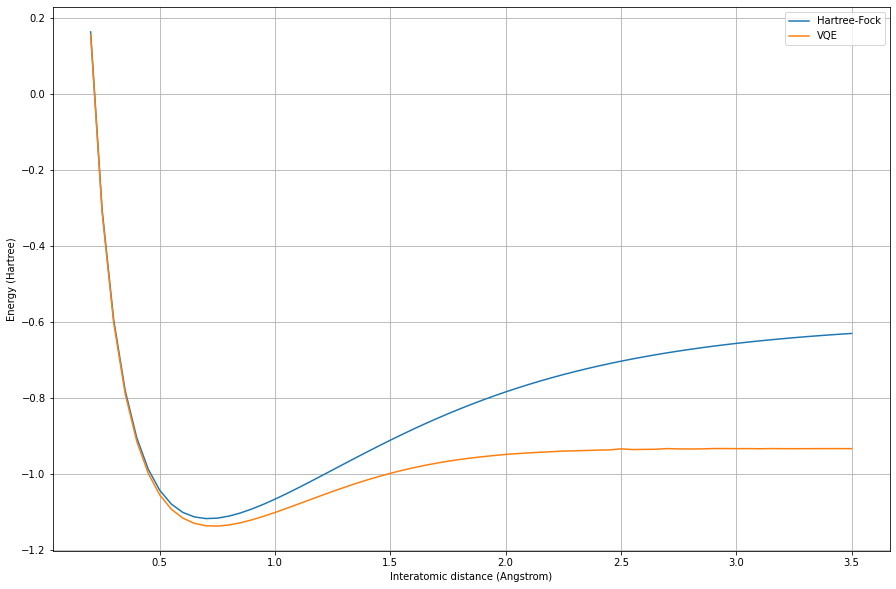
\includegraphics[width=1.0\textwidth]{Images/Capitolo3/Plots/H2_twolocal_ry_rz_cz_aer_cpu_plot.png}
    \captionof{figure}[Grafico 2 \newline TwoLocal - L\_BFGS\_B - Notebook\_CPU - Aer.]{}
    \label{fig:notebookcpu_twolocal_aer}
\end{minipage}
\begin{figure}[h]
    \begin{subfigure}[h]{0.49\linewidth}
        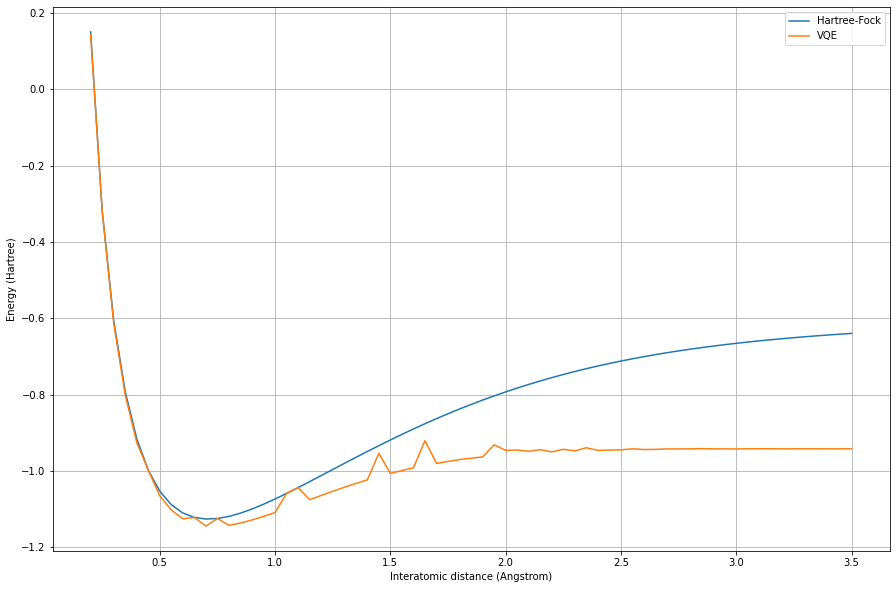
\includegraphics[width=0.80\linewidth]{Images/Capitolo3/Plots/H2_efficientsu2_linear_aer_cpu_plot.png}
        \caption{Linear}
    \end{subfigure}
    \hfill
    \begin{subfigure}[h]{0.49\linewidth}
        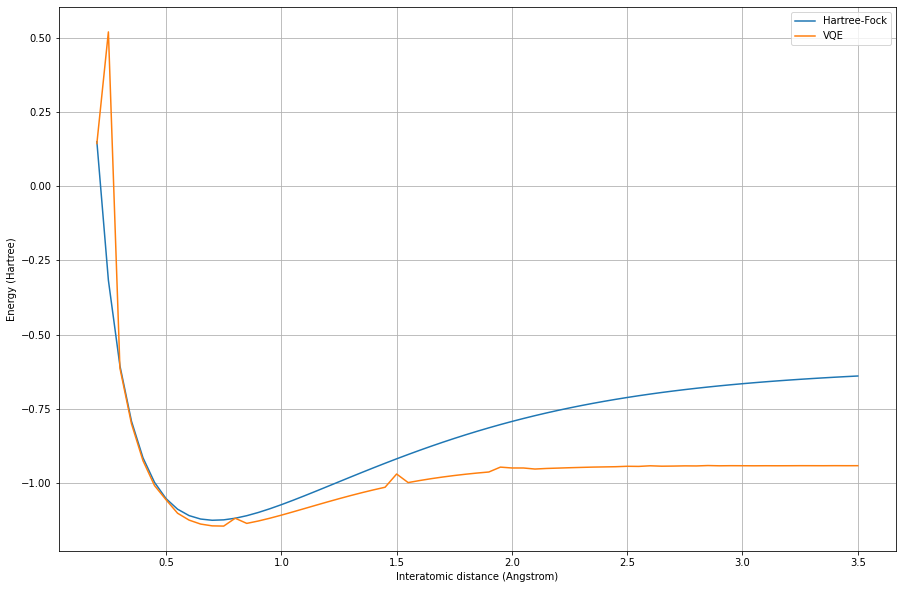
\includegraphics[width=0.80\linewidth]{Images/Capitolo3/Plots/H2_efficientsu2_full_aer_cpu_plot.png}
        \caption{Full}
    \end{subfigure}%
    \caption[Grafico 3 \newline EfficientSU2 - L\_BFGS\_B - Notebook\_CPU - Aer.]{}
    \label{fig:notebookcpu_efficientsu2_aer}
\end{figure}
\newline
La seconda simulazione è stata eseguita su Notebook\_CPU sia con il circuito TwoLocal che EfficientSU2 (linear/full entanglement).
Guardando la Tabella \ref{table:notebookcpu_aer} possiamo subito notare come il backend Aer abbia inciso nei tempi di esecuzione rispetto alla simulazione precedente ed anche in questo caso il grafico mostrato in Figura \ref{fig:notebookcpu_twolocal_aer} non presenta differenze sostanziali da quello desiderato.
Diverso è invece per il secondo circuito (\ref{fig:notebookcpu_efficientsu2_aer}) che pur avendo tempi di esecuzione minori, presenta molteplici picchi.
%-------------------------------------------------------------------------------------------------------
% TERZO TEST - Colab_CPU - Aer
\begin{minipage}[b]{0.39\textwidth}
    \scalebox{0.7}{%
    \begin{tabular}[b]{l|c}
        \hline\hline
        \multicolumn{2}{c}{\textbf{\textit{Colab\_CPU - Aer}}}\\
        \hline
        \multirow{3}{*}{\textit{TwoLocal}} & 21:16,5351521968842\\
        \cline{2-2} & 23:56,1901756127675\\
        \cline{2-2} & 23:26,9021610418955\\
        \hline\hline
    \end{tabular}}
    \captionsetup{type=table}
    \caption[Risultati terza simulazione.]{Nella colonna di destra sono riportati i tempi di esecuzione.}
    \label{table:colabcpu_aer}
\end{minipage}
\hfill
\begin{minipage}[b]{0.57\textwidth}
    \centering
    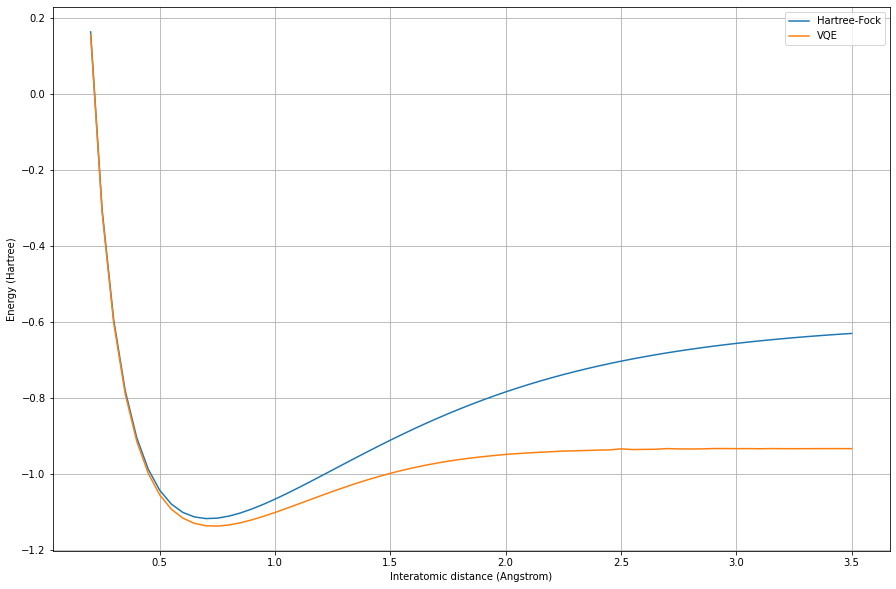
\includegraphics[width=1.0\textwidth]{Images/Capitolo3/Plots/H2_twolocal_ry_rz_cz_aer_cpu_plot.png}
    \captionof{figure}[Grafico 4 \newline TwoLocal - L\_BFGS\_B - Colab\_CPU - Aer.]{}
    \label{fig:colabcpu_twolocal_aer}
\end{minipage}
% Stesso plot di twolocal_ry_rz_cz_aer_cpu
\newline
La terza simulazione è stata eseguita su Colab\_CPU con il solo circuito TwoLocal e backend Aer.
I tempi ottenuti con la macchina messa a disposizione da Google, visibili nella Tabella \ref{table:colabcpu_aer}, sono risultati di poco peggiori rispetto ai test precedenti.
Il grafico, visibile in Figura \ref{fig:colabcpu_twolocal_aer}, rispecchia allo stesso modo il risultato atteso.
\newline\newline
%-------------------------------------------------------------------------------------------------------
% QUARTO TEST - Notebook_GPU - Aer
\begin{minipage}[b]{0.39\textwidth}
    \scalebox{0.7}{%
    \begin{tabular}[b]{l|c}
        \hline\hline
        \multicolumn{2}{c}{\textbf{\textit{Notebook\_GPU - Aer}}}\\
        \hline
        \multirow{3}{*}{\textit{TwoLocal}} & 20:28,53897968928\\
        \cline{2-2} & 20:41,6204098860423\\
        \cline{2-2} & 20:37,403276761373\\
        \hline
        \multirow{3}{6em}{\textit{EfficientSU2 (linear)}} & 13:14,5505837599437\\
        \cline{2-2} & 12:58,8811322053273\\
        \cline{2-2} & 12:27,9368682702382\\
        \hline
        \multirow{3}{6em}{\textit{EfficientSU2 (full)}} & 13:41,7947971820832\\
        \cline{2-2} & 13:39,1802767912546\\
        \cline{2-2} & 13:37,501518726349\\
        \hline\hline
    \end{tabular}}
    \captionsetup{type=table}
    \caption[Risultati quarta simulazione.]{Nella colonna di destra sono riportati i tempi di esecuzione.}
    \label{table:notebookgpu_aer}
\end{minipage}
\hfill
\begin{minipage}[b]{0.57\textwidth}
    \centering
    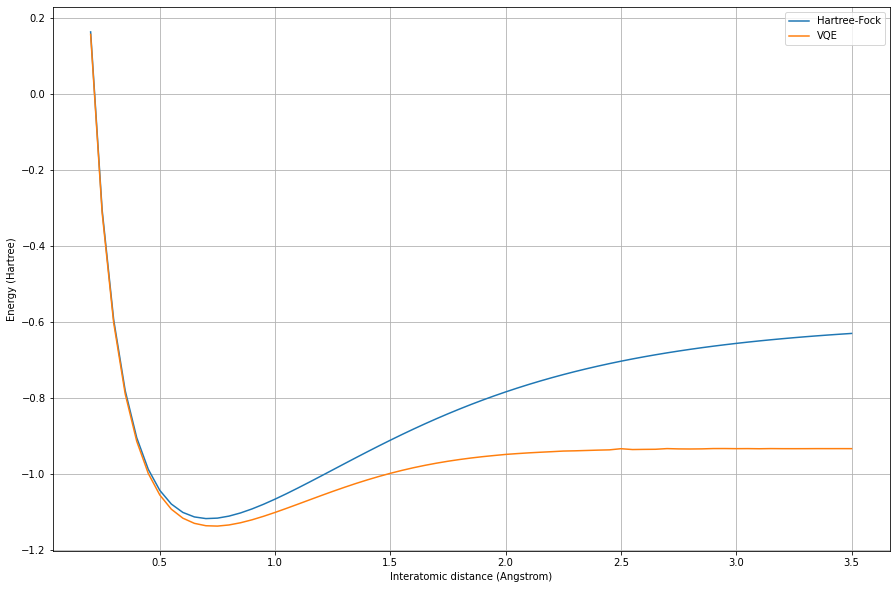
\includegraphics[width=1.0\textwidth]{Images/Capitolo3/Plots/H2_twolocal_ry_rz_cz_aer_gpu_plot.png}
    \captionof{figure}[Grafico 5 \newline TwoLocal - L\_BFGS\_B - Notebook\_GPU - Aer.]{}
    \label{fig:notebookgpu_twolocal_aer}
\end{minipage}
\begin{figure}[t]
    \begin{subfigure}[h]{0.49\linewidth}
        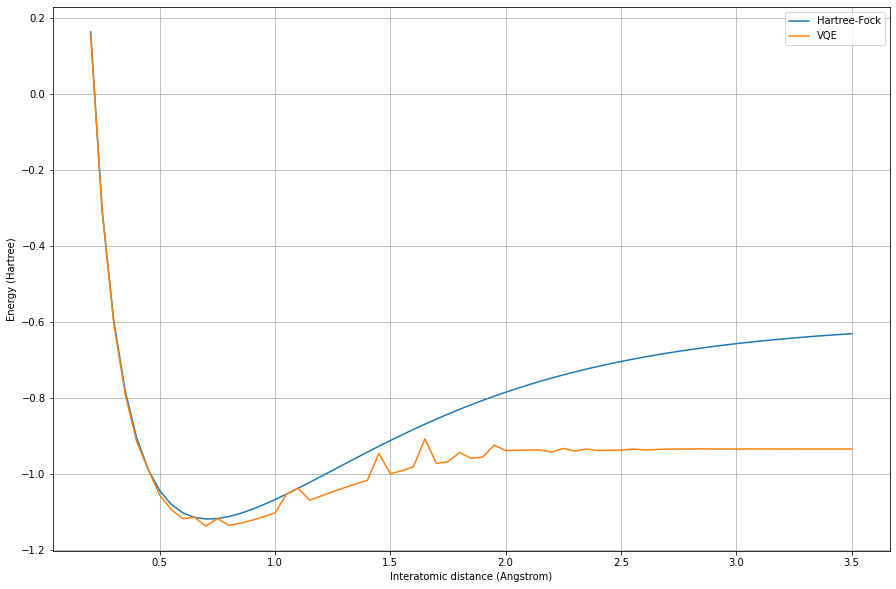
\includegraphics[width=\linewidth]{Images/Capitolo3/Plots/H2_efficientsu2_linear_aer_gpu_plot.png}
        \caption{Linear}
    \end{subfigure}
    \hfill
    \begin{subfigure}[h]{0.49\linewidth}
        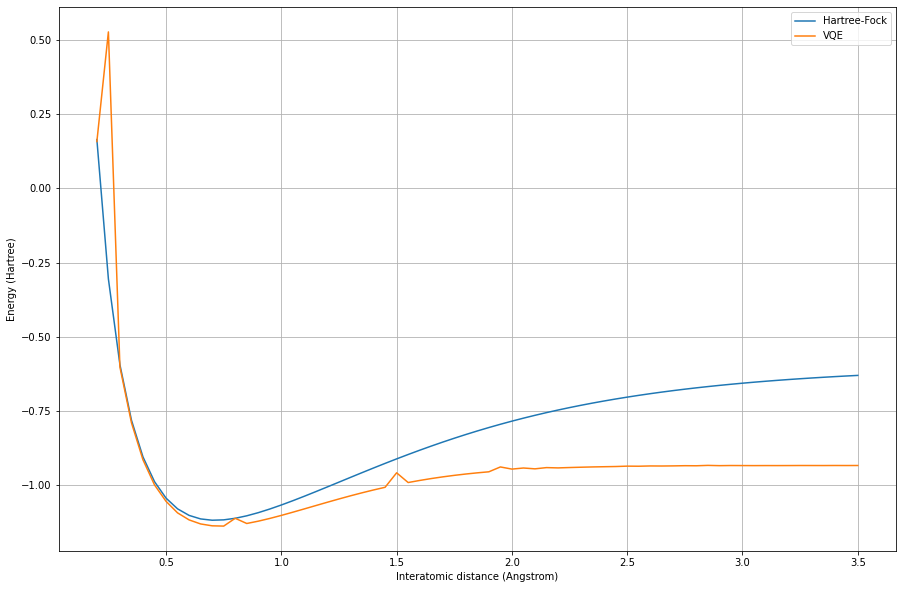
\includegraphics[width=\linewidth]{Images/Capitolo3/Plots/H2_efficientsu2_full_aer_gpu_plot.png}
        \caption{Full}
    \end{subfigure}%
    \caption[Grafico 6 \newline EfficientSU2 - L\_BFGS\_B - Notebook\_GPU - Aer.]{}
    \label{fig:notebookgpu_efficientsu2_aer}
\end{figure}
\newline\newline
Nella quarta simulazione abbiamo iniziato ad utilizzare la GPU, aspettandoci quindi dei tempi di esecuzione inferiori.
Purtroppo così non è stato, come si può notare dalla Tabella \ref{table:notebookgpu_aer}.
Il test è stato eseguito su Notebook\_GPU con entrambi i circuiti e backend Aer, i grafici mostrati nelle Figure \ref{fig:notebookgpu_twolocal_aer} e \ref{fig:notebookgpu_efficientsu2_aer} rimangono i medesimi visti in precedenza.
%-------------------------------------------------------------------------------------------------------

Per verificare che effettivamente questi risultati non dipendano dalla scarsa potenza della scheda video presente in Notebook\_GPU, abbiamo voluto effettuare uno stesso test su macchine teoricamente più prestanti.
%-------------------------------------------------------------------------------------------------------
% QUINTO TEST - Colab_GPU - Aer and Tower_GPU - Aer
\begin{table}[htp]
    \begin{subtable}[h]{0.45\textwidth}
        \centering
        \scalebox{0.9}{
        \begin{tabular}{l|c}
            \hline\hline
            \multicolumn{2}{c}{\textbf{\textit{Colab\_GPU - Aer}}}\\
            \hline
            \multirow{3}{*}{\textit{TwoLocal}} & 25:03,993593454361\\
            \cline{2-2} & 25:03,7793548901875\\
            \cline{2-2} & 25:33,4875607490538\\
            \hline\hline
        \end{tabular}}
       \caption{}
       \label{table:colabgpu_aer}
    \end{subtable}
    \hfill
    \begin{subtable}[h]{0.45\textwidth}
        \centering
            \scalebox{0.9}{
            \begin{tabular}{l|c}
            \hline\hline
            \multicolumn{2}{c}{\textbf{\textit{Tower\_GPU - Aer}}}\\
            \hline
            \multirow{3}{*}{\textit{TwoLocal}} & 01:36:05,113420333332\\
            \cline{2-2} & 01:50:58,047812833333\\
            \cline{2-2} & 01:39:39,373367333333\\
            \hline\hline
        \end{tabular}}
        \caption{}
        \label{table:towergpu_aer}
     \end{subtable}
     \caption[Risultati quinta simulazione.]{Nella colonna di destra sono riportati i tempi di esecuzione.}
\end{table}
\newline

Si può notare dai risultati delle Tabelle \ref{table:colabgpu_aer} e \ref{table:towergpu_aer} come l'effettiva potenza di calcolo della GPU non incida nei tempi di esecuzione e che piuttosto sia la CPU a fare da padrona.
Probabilmente nella macchina Tower\_GPU, oltre ad avere un processore meno prestante, ha inciso il fatto di utilizzare Ubuntu su WSL2 e di conseguenza, essendo un ambiente virtualizzato, non si ha piena comunicazione con l'hardware.
%-------------------------------------------------------------------------------------------------------
% SESTO TEST - Notebook_GPU - Aer - LiH

Infine, prima di passare all'utilizzo di altri ottimizzatori, si vuole mostrare l'unico test svolto sulla molecola d'Idruro di Litio ($LiH$) che ha richiesto tempi d'esecuzione ben più lunghi, senza nemmeno portare a dei buoni risultati.
\begin{figure}[h]
    \begin{subfigure}[h]{0.49\linewidth}
        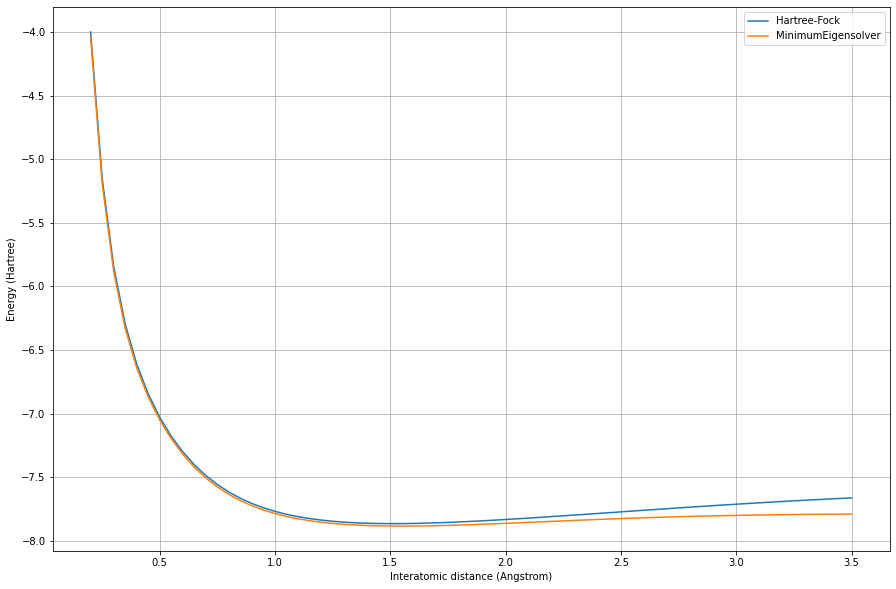
\includegraphics[width=\linewidth]{Images/Capitolo3/Plots/LiH_numpy_minimum_eigensolver_plot.png}
        \caption{NumpyMinimumEigensolver}
    \end{subfigure}
    \hfill
    \begin{subfigure}[h]{0.49\linewidth}
        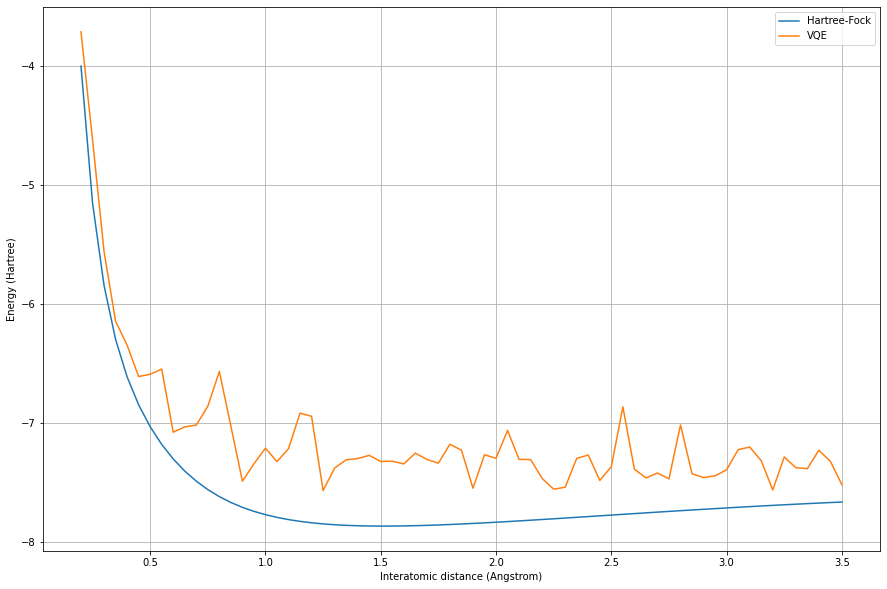
\includegraphics[width=\linewidth]{Images/Capitolo3/Plots/LiH_twolocal_ry_rz_cz_gpu_plot.png}
        \caption{VQE}
    \end{subfigure}%
    \caption[Grafico 7 \newline LiH - TwoLocal - L\_BFGS\_B - Notebook\_GPU - Aer.]{}
    \label{fig:notebookgpu_LiH_aer}
\end{figure}

La sesta simulazione è stata svolta su Notebook\_GPU, con circuito TwoLocal e backend Aer.
I tempi di esecuzione per l'algoritmo VQE si aggirano intorno alle 19 ore e dal grafico di destra si può notare come il risultato non sia per nulla soddisfacente.
%-------------------------------------------------------------------------------------------------------
\subsubsection{Altri ottimizzatori}
L'utilizzo del circuito TwoLocal ci ha permesso di ottenere i risultati migliori, pertanto di seguito verranno mostrate le ultime simulazioni svolte su backend Aer, dove si ricorre ad altri tipi di ottimizzatori.
\newline\newline
\begin{minipage}[b]{0.39\textwidth}
    \scalebox{0.8}{%
    \begin{tabular}[b]{l|c}
        \hline\hline
        \multicolumn{2}{c}{\textbf{\textit{Notebook\_GPU - COBYLA}}}\\
        \hline
        \multirow{3}{*}{\textit{TwoLocal}} & 20:28,53897968928\\
        \cline{2-2} & 20:41,6204098860423\\
        \cline{2-2} & 20:37,403276761373\\
        \hline\hline
    \end{tabular}}
    \captionsetup{type=table}
    \caption[Risultati simulazione COBYLA.]{Nella colonna di destra sono riportati i tempi di esecuzione.}
    \label{table:notebookgpu_cobyla_aer}
\end{minipage}
\hfill
\begin{minipage}[b]{0.57\textwidth}
    \centering
    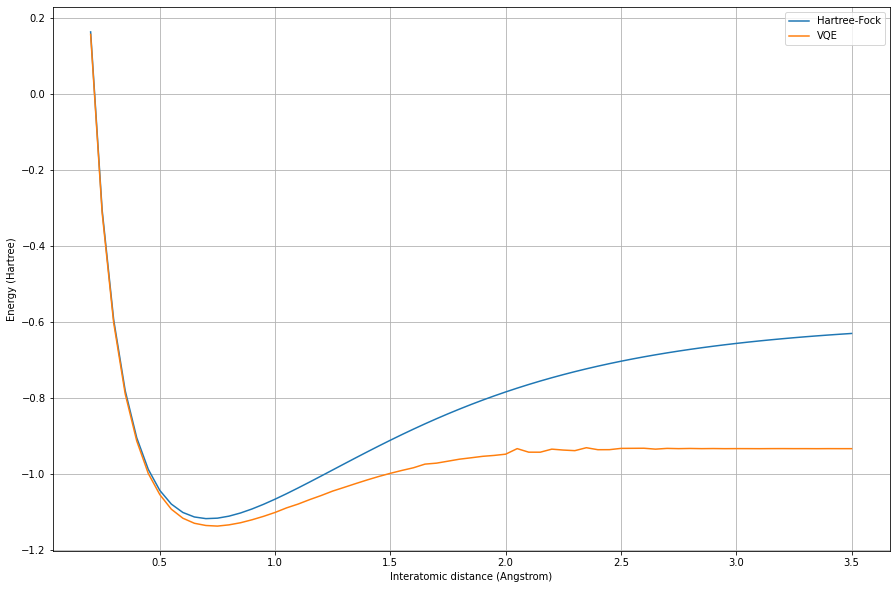
\includegraphics[width=1.0\textwidth]{Images/Capitolo3/Plots/H2_twolocal_ry_rz_cz_cobyla_aer_gpu_plot.png}
    \captionof{figure}[Grafico 8 \newline TwoLocal - COBYLA - Notebook\_GPU - Aer.]{}
    \label{fig:notebookgpu_twolocal_cobyla_aer}
\end{minipage}

I risultati sopra evidenziati (Tabella \ref{table:notebookgpu_cobyla_aer}), inerenti la simulazione svolta su Notebook\_GPU utilizzando il circuito TwoLocal e l'ottimizzatore COBYLA, mostrano dei tempi di esecuzione molto simili ai precedenti. Nel grafico in Figura \ref{fig:notebookgpu_twolocal_cobyla_aer} è possibile vedere delle piccole increspature che non vanno ad incidere notevolmente sull'esito del test.
\newline
\begin{minipage}[b]{0.39\textwidth}
    \scalebox{0.8}{%
    \begin{tabular}[b]{l|c}
        \hline\hline
        \multicolumn{2}{c}{\textbf{\textit{Notebook\_GPU - SPSA}}}\\
        \hline
        \multirow{3}{*}{\textit{TwoLocal}} & 44:13,694082101186\\
        \cline{2-2} & 44:37,829064130783\\
        \cline{2-2} & 46.12,1066045761106\\
        \hline\hline
    \end{tabular}}
    \captionsetup{type=table}
    \caption[Risultati simulazione SPSA.]{Nella colonna di destra sono riportati i tempi di esecuzione.}
    \label{table:notebookgpu_spsa_aer}
\end{minipage}
\hfill
\begin{minipage}[b]{0.57\textwidth}
    \centering
    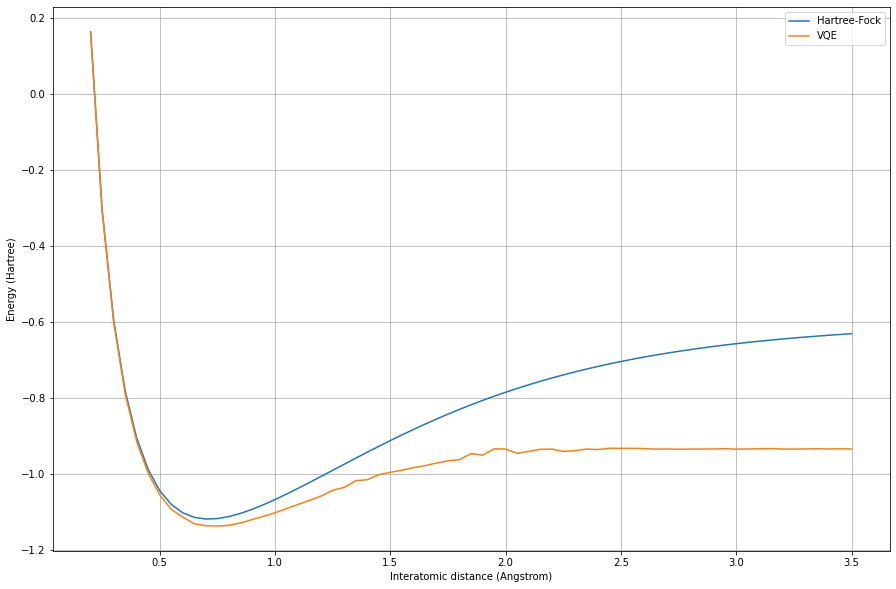
\includegraphics[width=1.0\textwidth]{Images/Capitolo3/Plots/H2_twolocal_ry_rz_cz_spsa_aer_gpu_plot.png}
    \captionof{figure}[Grafico 9 \newline TwoLocal - SPSA - Notebook\_GPU - Aer.]{}
    \label{fig:notebookgpu_twolocal_spsa_aer}
\end{minipage}

Un'ulteriore simulazione è stata fatta utilizzando l'ottimizzatore SPSA.\newline
Come si può vedere nella Tabella \ref{table:notebookgpu_spsa_aer} i tempi di esecuzione risultano raddoppiati ed anche il grafico, mostrato in Figura \ref{fig:notebookgpu_twolocal_spsa_aer}, presenta qualche imperfezione in più.
\begin{figure}[htp]
    \centering
    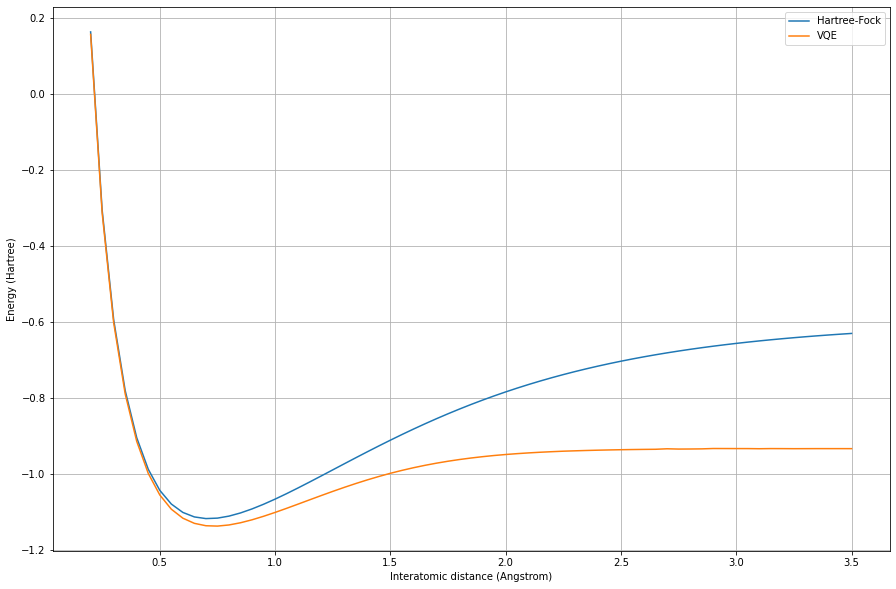
\includegraphics[width=8cm]{Images/Capitolo3/Plots/H2_twolocal_ry_rz_cz_slsqp_aer_gpu_plot.png}
    \caption[Grafico 10 \newline TwoLocal - SLSQP - Notebook\_GPU e Colab\_GPU - Aer.]{}
    \label{fig:notebookgpu_twolocal_slsqp_aer}
\end{figure}
\begin{table}[h]
    \begin{subtable}[h]{0.45\textwidth}
        \centering
        \begin{tabular}[b]{l|c}
            \hline\hline
            \multicolumn{2}{c}{\textbf{\textit{Notebook\_GPU - SLSQP}}}\\
            \hline
            \multirow{3}{*}{\textit{TwoLocal}} & 22:49,5642606417338\\
            \cline{2-2} & 22:51,5691443284354\\
            \cline{2-2} & 21:10,095632870992\\
            \hline\hline
        \end{tabular}
        \caption{}
        \label{table:notebookgpu_slsqp_gpu}
    \end{subtable}
    \hfill
    \begin{subtable}[h]{0.45\textwidth}
        \centering
        \begin{tabular}[b]{l|c}
            \hline\hline
            \multicolumn{2}{c}{\textbf{\textit{Colab\_GPU - SLSQP}}}\\
            \hline
            \multirow{3}{*}{\textit{TwoLocal}} & 26:19,887064695358\\
            \cline{2-2} & 38:01,3527413209276\\
            \cline{2-2} & 26:39,4683996836343\\
            \hline\hline
        \end{tabular}
        \caption{}
        \label{table:colabgpu_slsqp_gpu}
     \end{subtable}
     \caption[Risultati simulazioni SLSQP.]{Nella colonna di destra sono riportati i tempi di esecuzione.}
\end{table}

Come ultimo ottimizzatore è stato utilizzato SLSQP e sono state svolte rispettivamente due simulazioni: la prima riguarda Notebook\_GPU, che è riuscita ad ottenere dei risultati (Tabella \ref{table:notebookgpu_slsqp_gpu}) paragonabili a L\_BFGS\_B con dei tempi di esecuzione molto simili; la seconda riguarda Colab\_GPU, dove i tempi di esecuzione, mostrati nella Tabella \ref{table:colabgpu_slsqp_gpu}, sono di poco superiori.
Uno dei tre test riguardanti questa macchina è stato svolto più volte ma non si è potuto notare un miglioramento.

Entrambe le macchine hanno ottenuto un buon grafico (Figura \ref{fig:notebookgpu_twolocal_slsqp_aer}), molto simile a quello atteso calcolato dall'algoritmo classico NumpyMinimumEigensolver.